\documentclass[a4paper,11pt]{article}
\usepackage{amsmath}
\usepackage{amssymb}
\usepackage{graphicx}
\usepackage{verbatim}
\author{William Song}
\title{Tex from Anywhere}

\begin{document}

%\maketitle title author datetime

\tableofcontents


	\section{Hello Anywhere} u can write tex\\ from anywhere
		\subsection{MikTex} MikTex on
Windows
			\subsubsection{CTex}CTex integrate MikTex
				\paragraph{Editor}TeXworks
					\subparagraph{2 windows}one for edit one for review
		\subsection{Emacs}Emacs on Linux
			\subsubsection{Emacs-LaTex}use Emacs-LaTex inside
\newline

\LaTeX2e \newline

\# \$ \% \^{O} \& \_ \{ \}   \~{A}

 $\backslash$

Today is \today

\begin{comment}
so, so
you think
you can tell
heaven from hell
\end{comment}
A
\\
\\
\\
\\
\\
\\%awlful... break pages
\\
\\
\\
\\
\\
	\section{math}The Newton's second law is F=ma. %\\The Newton's second law is $F=ma$.  %\\just slice current line, and continue format-type?

	\paragraph{in} The Newton's second law is $F=ma$. % $$F=ma$$

	The Newton's second law is \[F=ma\].  %\\  %\\ can use independently to influence current line and next line's format
	x\\
	y\\
	z

	\paragraph{in}
	Greek Letters $\eta$ and $\mu$.
%empty line start new box format  %\\ in fact continue inbox format, just like line-break...
	Fraction $\frac{a}{b}$

	Power $a^b$

	Subscript $a_b$\\
	Derivate $\frac{\partial y}{\partial t}$\\
	Vector $\vec{n}$\\
	Bold $\mathbf{n}$\\
	To time differential $\dot{F}$\\
	Matrix (lcr here means left , center or right for each column)
	\[
		\left[
			\begin{array}{llcr}
				a1 & b22 & c333 & mrrr\\
				d444 & e55555 & f6 & Po\\
%				I111  %llcr columns, just so so. llcr 4cols, l 1col...
			\end{array}
		\right]
	\]

	Equations(here \& is the symbol for aligning different rows)
	\begin{align}
		a+b&=c\\
		d=e+f&+g
	\end{align}

	\[
		\left\{ %note \{   in  \[
			\begin{aligned}
				&a+b=c\\
				&d=e+f+g\\
				&h=i+j
			\end{aligned} %aligned diff align
		%\right\}%right. for what?
			\begin{aligned}
				&I \\
				&II\\
				&III
			\end{aligned}
		\right\}%right. for what?
	\]
	
	\begin{center}
%	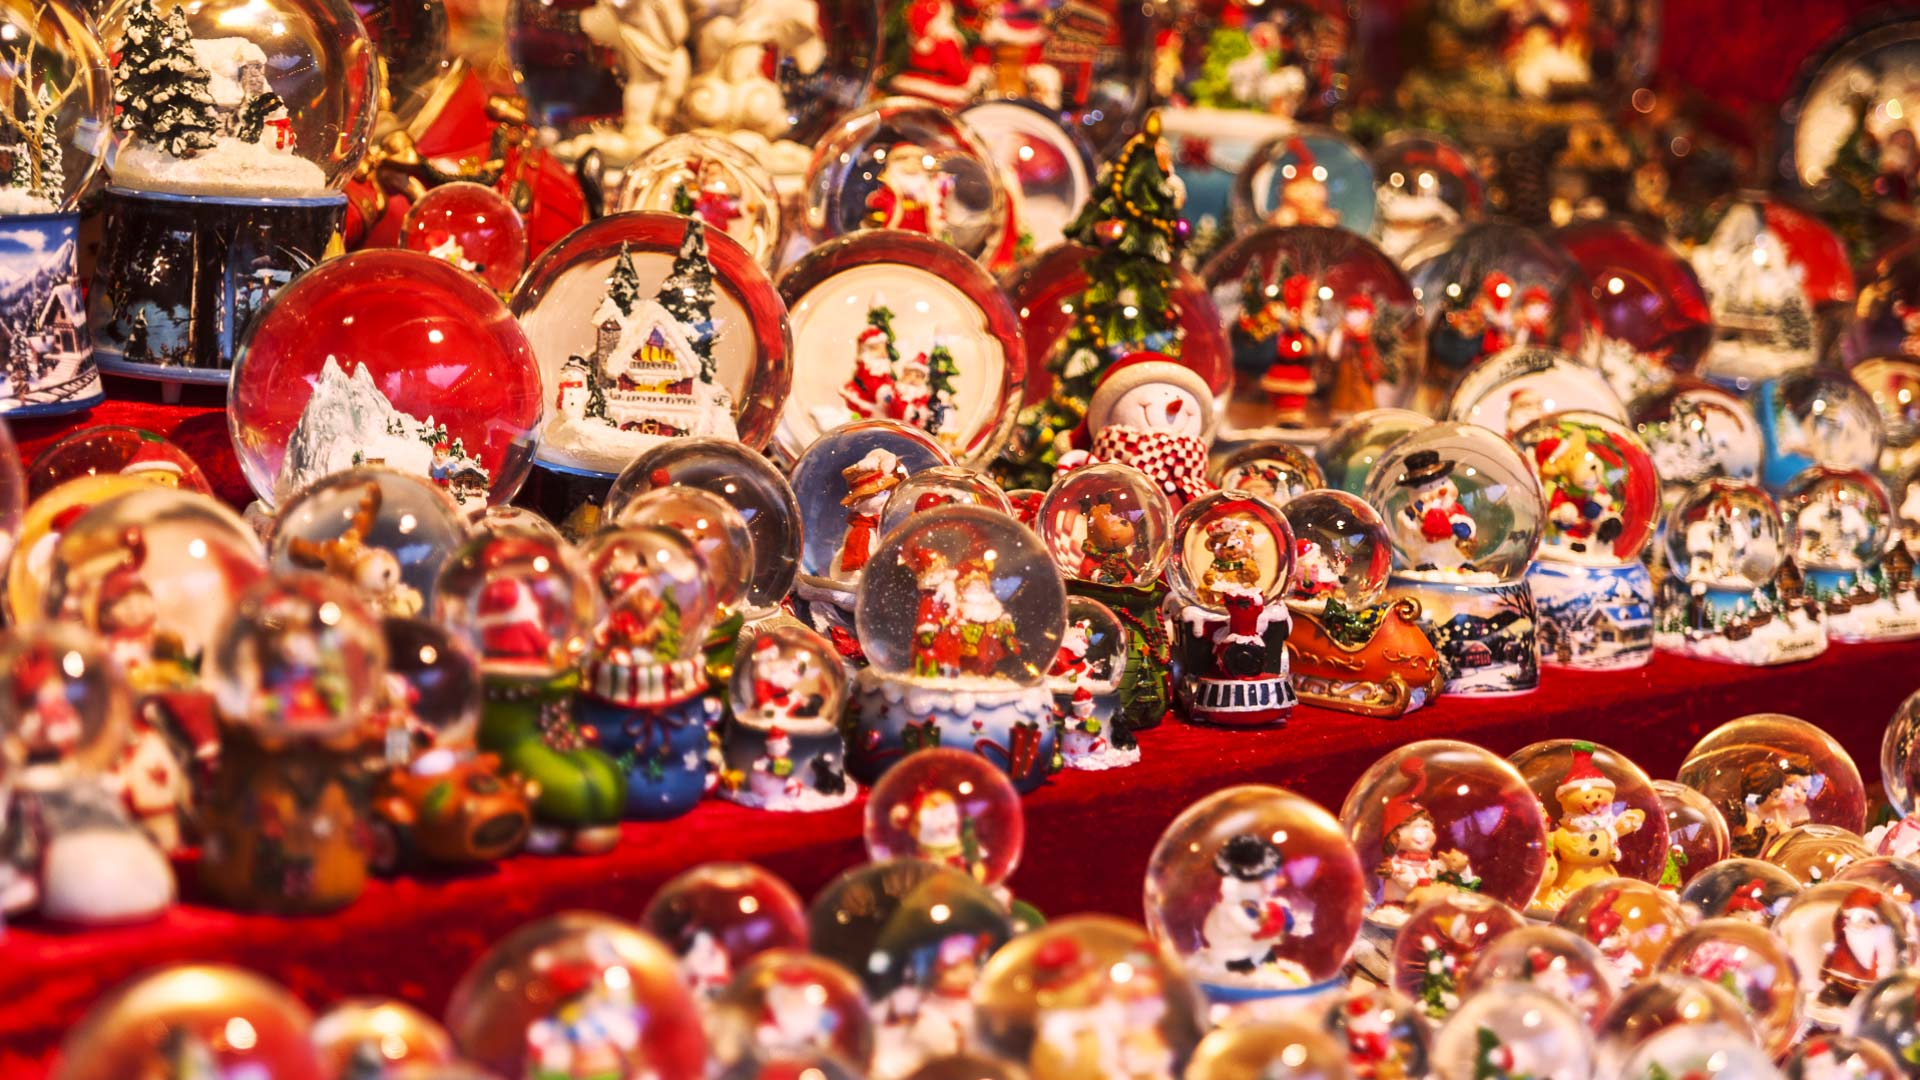
\includegraphics[width=7.00in,height=4.00in]{1,eps.jpg}
	\end{center}


	\begin{tabular}{ll|}
		%\cline{1-2}
		\hline
		\vline a1 &  \vline b21 \\
		c321 & d54321 \\
	\end{tabular}
	\begin{tabular}{|c|c|}
		\hline
		a & b \\
		\hline
		c & d \\
		\hline
	\end{tabular}	
	\begin{center}
		\begin{tabular}{|c|c|}
			\hline
			a & b \\ \hline
			c & d \\
			\hline
		\end{tabular}
	\end{center}

    \begin{tabular}{|c|c|c|}
      \hline
      % after \\: \hline or \cline{col1-col2} \cline{col3-col4} ...
      1 & 0 & 0 \\ \hline
      0 & 2 & 3 \\ \hline
      0 & 1 & 1 \\
      \hline
    \end{tabular}
	
	\begin{tabular}{|r|}
	•Q
	\end{tabular}•

\end{document}
















